%%
%% This is file `kaumasterstemplate.tex',
%% generated with the docstrip utility.
%%
%% The original source files were:
%%
%% kauthesis.dtx  (with options: `masterstemplate')
%% 
%% This is a generated file.
%% 
%% Copyright (c) 2011-2014 Stefan Berthold <stefan.berthold@kau.se>
%% 
%% This file is part of the kauthesis bundle.
%% 
%% This work may be distributed and/or modified under the
%% conditions of the LaTeX Project Public License, either version 1.3
%% of this license or (at your option) any later version.
%% The latest version of this license is in
%%   http://www.latex-project.org/lppl.txt
%% and version 1.3 or later is part of all distributions of LaTeX
%% version 2005/12/01 or later.
%% 
%% This work has the LPPL maintenance status `author-maintained'.
%% 
%% The Current Maintainer and author of this work is Stefan Berthold.
%% 
%% This work consists of all files listed in manifest.txt.
%% 
%% kauthesis.dtx
%% Copyright (c) 2011-2015 Stefan Berthold <stefan.berthold@kau.se>
\documentclass{kaumasters} % available class options: garamond
\usepackage[swedish]{babel}
\usepackage[T1]{fontenc}
\usepackage[utf8]{inputenc}
\usepackage{titletoc}
\usepackage{geometry}
\usepackage{booktabs}

%% break long URLs in references.
\usepackage{url}
\def\UrlBreaks{\do\/\do-}
% list
\usepackage{scrextend}
\addtokomafont{labelinglabel}{\sffamily}

\usepackage{fancyhdr}

\usepackage{graphicx}
\graphicspath{{../figures/background/}}
\usepackage[numbers]{natbib}

\renewcommand{\baselinestretch}{1.5} 


\makeatletter
\renewcommand\scriptsize{\@setfontsize\scriptsize{7}{8}}
\renewcommand\tiny{\@setfontsize\tiny{5}{6}}
\renewcommand\small{\@setfontsize\small{5}{6}}
\renewcommand\normalsize{\@setfontsize\normalsize{12}{12}}
\renewcommand\large{\@setfontsize\large{10.95}{15}}
\renewcommand\Large{\@setfontsize\Large{12}{16}}
\renewcommand\LARGE{\@setfontsize\LARGE{14.4}{18}}
\renewcommand\huge{\@setfontsize\huge{20.74}{30}}
\renewcommand\Huge{\@setfontsize\Huge{24}{36}}
\makeatother
\usepackage{sectsty}

\chapterfont{\Huge}
\sectionfont{\huge}
\subsectionfont{\LARGE}
\subsubsectionfont{\Large}
\paragraphfont{\Large}


%\pagestyle{fancy}
%\fancyhf{}
%\lhead[\texttit{}]{}
%\rhead[]{}
%\setlength{\headheight}{15pt}

\title{Twitter Sentiment Analysis}
\author{Johan Selberg, Johannes Bandgren}
\supervisor{Kerstin Andersson}
\examiner{Exam}
\institute{Department of Computer Science}
\place{Karlstad Universitet}
\begin{document}

\maketitle



\frontmatter
\begin{abstract}
  Abstract.
  \keywords keywords
\end{abstract}
\approvalpage%
\begin{acknowledgements}
  Thanks.
\end{acknowledgements}

\tableofcontents{}
\listoffigures
\listoftables
\mainmatter
% för att fucka med marginaler
%\newgeometry{top=20mm, bottom=20mm, right=30mm, left=30mm}
\pagestyle{fancy}
\fancyhead[LE,RO]{\thepage}
\fancyhead[RE,LO]{\rightmark}
\fancyfoot{}
\chapter{Introduktion}

\newpage


\chapter{Bakgrund}
\section{Introduktion}
Syftet med studien är att utvärdera (x) stycken klassificeringsmodeller inom maskininlärning och hur bearbetningen samt märkningen av en datamängd påverkar en klassificeringsmodells prestanda. Maskininlärningsalgoritmerna som kommer användas för att fram klassiciferingsmodellerna är Naive Bayes, Support Vector Machine och ZZZZZ. Figur \ref{fig:overfig} visar en förenklad överblick hur processen för att utvärdera klassificeringsmodellerna kommer se ut. Datamängden består utav en mängd indata som är märkt med förväntad utdata, som går igenom en bearbetningsprocess där t.ex. data som inte tillför något värde tas bort och där mängden av data delas upp i tränings- och valideringsdata.  Bearbetningsprocessen diskuteras mer ingående i \ref{exp:pre}. På den bearbetade datan utförs ett särdragsurval, där dataspecifika särdrag plockas ut…MER .. som diskuteras vidare i \ref{exp:feat}. Träningsmängden används av maskininlärningsalgoritmen för att skapa klassiciferingsmodellen. När klassificeringsmodellen är framtagen används valideringmängden för att utvärdera prestandan av modellen.

\begin{figure}[h]
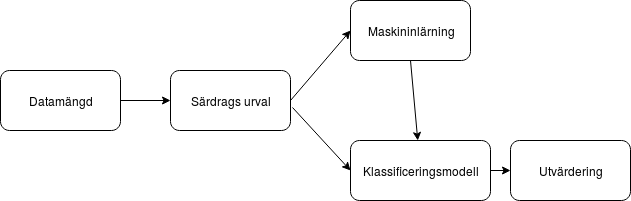
\includegraphics[width=12cm]{oversiktsfigur}
\centering
\caption{Utvärderingsprocessen av maskininlärningsmodeller}
\label{fig:overfig}
\end{figure}

Studien kommer använda maskininlärning för att utföra sentimentanalys (SA) d.v.s utläsa huruvida en text uttrycker någonting positivt eller negativt. Uppdragsgivaren, CGI, betraktar sentimentanalys  som en viktig pusselbit för framtida lösningar dem vill erbjuda sina kunder. Lösningar skulle kunna vara chatbotar där sentimentanalys används så att chatboten ändrar sitt språk utefter svaren från slutanvändare. Eller att det kan användas för trendanalys där ett företag vill veta vad allmänheten tycker före och efter att man har släppt en ny produkt eller efter att kvartalsrapporten har släppts.

I avsnitt \ref{SA} förklaras vad SA är och under \ref{SAkt} beskrivs dem olika klassificeringsteknikerna inom SA.
I avsnitt \ref{ML} ges en kort introduktion till maskininlärning och framstegen som gjort under den senaste tiden. I avsnitt \ref{MLvised} beskrivs hur inlärningprocessen kan utföras och avsnitt \ref{MLsvm} och \ref{MLnb} förklarar kort hur NB, SVM och XXX fungerar. I avsnitt \ref{DS} ges en överblick hur en datamängd ser ut och vilka märkningsmetoder som används för twittersentimentanalys (TSA), medans i avsnitt \ref{DSse} och \ref{DSsts} beskrivs de valda datamängderna. I avsnitt \ref{TSA} ges en introduktion till TSA. Medan i avsnitten \ref{TSAchall} och \ref{TSAprob} beskrivs utmaningar och problem med TSA. Sluligen i avsnitt \ref{TSAev} förklaras vilka hjälpmedel som kommer användas för att utvärdera algoritmernas prestanda.


\section{Sentimentanalys} \label{SA}
SA används för att studera människors åsikter, attityder och känslor mot andra entiteter. En entitet kan vara ett ämne, en händelse eller en individ. Målet med SA är att identifiera känslan som är uttryckt i en text för att därefter analysera den. Processen delas upp i tre steg: att hitta åsikter, identifiera känslan för de åsikterna och slutligen klassificera motsatsförhållandet dem emellan \cite{SAsurvey}.

Inom SA appliceras klassificeringen på 3 olika nivåer: dokument-, menings- och aspektnivå \cite{SAsurvey}. SA på dokumentnivå klassificerar om ett helt dokument uttrycker en positiv eller negativ åsikt, exempel på dokument kan vara produktrecensioner eller nyhetsartiklar. Medan på meningsnivå klassificeras varje mening i ett dokument. Slutligen nere på aspektnivå analyseras de möjliga aspekterna av en entitet. En mening kan behandla olika aspekter av en entitet. Både positiva och negativa åsikter kan delges om en entitets olika aspekter. Ett exempel på det är meningen “Ölen var väldigt god, men tyvärr alldeles för dyr”, som innehåller både en positiv och en negativ åsikt om en entitet som i det här fallet är ölen.
\subsection{Klassificeringstekniker} \label{SAkt}
De olika klassificeringsteknikerna som i nuläget används för SA delas upp i 3 olika kategorier: maskininlärningsmetoder, lexikonbaserade metoder samt hybrida metoder \cite{SAsurvey}. 

Maskininlärningsmetoder använder etablerade maskininlärningsalgoritmer tillsammans med språkliga särdrag för att konstruera klassificerare som kan avgöra om en text uttrycker någonting positivt eller negativt [ref=Sentiment analysis a survey]. Prestandan för maskininlärningsmetoder är beroende av mängden träningsdata, större mängder data ger vanligtvis bättre resultat \cite{TSAsurvey}. Maskininlärningsmetoder är dessutom domänberoende, vilket gör att de inte presterar bra när de används på andra domän än det de har tränats på. 

Lexikonbaserade metoder använder sig av ordlistor för att analysera text \cite{SAsurvey}. Ordlistorna består av positiva och negativa termer som används för att beräkna vad en given text uttrycker för sentiment.
Fördelen med lexikonbaserade metoder är att de inte kräver någon  träningsdata \cite{TSAsurvey}. Men faktumet att de är beroende av statiska ordlistor betyder att de inte tar hänsyn till termer som inte finns i ordlistorna. Det betyder att ordlistor måste uppdateras kontinuerligt för innehåll som är dynamiskt och ständigt under utveckling, vilket är särskilt problematisk för texter som förekommer på sociala medier. 

Hybrida metoder kombinerar lexikonbaserade metoder med maskininlärningsmetoder \cite{TSAsurvey}. Genom att kombinera metoderna med varandra kan de väga upp för varandras svagheter. Nackdelen med hybrida metoder är dock att de kräver en hög beräkningskomplexitet.

Experimentet som presenteras i studien fokuserar enbart på maskininlärningsmetoder.

\section{Maskininlärning} \label{ML}
Maskininlärning är ett delområde inom artificiell intelligens (AI), där målet är att göra det möjligt för datorer att lära sig på egen hand. Maskininlärningsalgoritmer gör det möjligt att identifiera olika mönster från observerad data, bygga upp en generell modell som kan förutsäga saker utan att ha blivit förprogrammerade med explicita regler för hur den ska lösa ett problem. Under de senaste åren har stora framsteg inom maskininlärning gjorts. Exempelvis utvecklade DeepMind \cite{DMatari00} 2015 en agent som mästrade 49 st Atari-spel \cite{wiki:004}, med en klassificeringsmodell med endast pixlar och spelpoäng som indata. Under 2016 utvecklade DeepMind sin AlphaGo \cite{DMgo} agent som besegrade en av världens bästa Go spelare, Lee Sedol \cite{wiki:005} med 4-1 i matcher. Detta var ett framsteg för AI eftersom Go är ett komplext spel med $2 * 10^{170}$ möjliga drag \cite{wiki:006}.

** förklara bredare tillämpningar **

%\section{Övervakad och oövervakad inlärning} \label{MLvised}
Figur \ref{fig:ml} illustrerar att maskininlärning delas upp i två typer av inlärningsprocesser dvs. i övervakad eller oövervakad inlärning och deras underliggande algoritmer.
\begin{figure}[h]
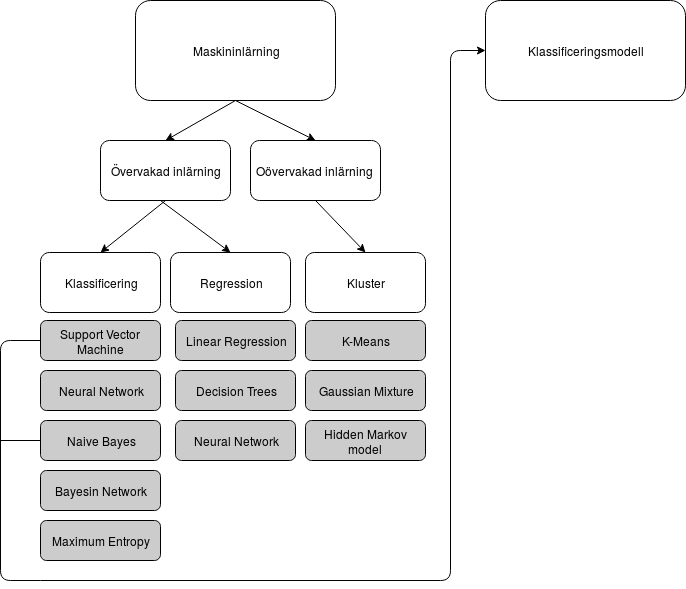
\includegraphics[width=12cm]{ml}
\centering
\caption{Inlärningsprocesser för maskininlärning.}
\label{fig:ml}
\end{figure}

Oövervakad inlärning används när datamängden bara består av indata och inget förväntat resultat. Målet med oövervakad inlärning är att algoritmen själv lär sig att modellera den komplexa underliggande strukturen så att den kan lära sig mer om datan och själv komma fram till ett resultat \cite{wiki:007}. Exempelvis kan en övervakad klusteralgoritm användas för att hitta likheter i bilder och gruppera dem följaktligen.
Övervakad inlärning används när datamängden består av både indata och dess förväntade utdata. Den övervakade algoritmen använder datamängden för att lära sig hur utdata beror på indata genom att skapa en klassificeringsmodell som används för att förutse utdata från ny indata som illustreras i figur \ref{fig:kl}. 
Övervakad inlärning kan man tänka sig som att en lärare övervakar programmets inlärningsprocess. Under inlärningsprocessen försöker algoritmen iterativt förutse utdata från datamängden och blir rättad av läraren vid fel förutsägelse \cite{learning:001}.

\begin{figure}[h]
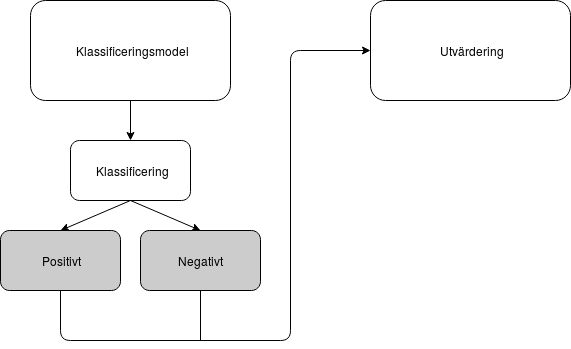
\includegraphics[width=12cm]{klassmodell}
\centering
\caption{Klassificeringsprocess av data.}
\label{fig:kl}
\end{figure}

Övervakad inlärning kan brytas ner till klassificerings- och regressionsproblem och eftersom TSA kan kallas ett typiskt klassificeringsproblem \cite{SAsurvey}, kommer studien att använda algoritmer lämpade för klassificeringsproblem. I figur \ref{fig:ml} kan vi se några utav dessa klassificeringsalgoritmer och enligt \cite{TSAsurvey} är speciellt Naive Bayes (NB) och Support Vector Machine (SVM) algoritmerna bäst lämpade för TSA.

\subsection{Naive Bayes} \label{MLnb}
NB är en klassificeringsalgoritm som är baserad på Bayes theorem \cite{wiki:009} med starka (“naive”) oberoende antaganden mellan särdragen d.v.s NB förutsätter att närvaron av ett visst särdrag i en klass inte relaterar till närvaron av ett annat särdrag. 
Exempelvis kan en frukt anses vara ett äpple om det är grönt, runt och är 10 cm i diameter. Även om särdragen grönt, runt och diameter beror på varandra eller på att dom existerar så bidrar alla särdragen självständigt till sannolikheten att frukten är ett äpple, det är därför algoritmen kallas (“naive”) \cite{nb:001}.

\subsection{Support Vector Machine} \label{MLsvm}
SVM är en övervakad maskininlärningsalgoritm som kan användas till både klassifikations- och regressionsproblem, för det mesta används SVM för klassifikationsproblem. SVM är baserat på iden att hitta ett hyperplan \cite{svm:001} som bäst delar upp datamängden till två klasser \cite{svm:003}. Givet en träningsmängd där förväntad utdata är markerad till en av två kategorier bygger SVM algoritmen upp en klassificeringsmodell som kan användas för att förutse vilken kategori ny indata ger \cite{svm:002}. 

\subsection{XXX}

\section{Datamängd} \label{DS}
En datamängd för övervakad inlärning består utav en mängd in- och utdata som diskuteras i sektion \ref{MLvised}. Processen för hur rätt udata (positivt/negativ) markeras till varje indata kan utföras på två olika sätt, antingen genom så kallad mänsklig märkning där människor markerar indata som positivt/negativ eller genom “distant supervision” där en dator märker indata som positivt/negativt utefter någon parameter. Den stora skillnaden mellan mänsklig märkning och “distant supervision” är att “distant supervision” kan generera en mycket större datamängd än mänsklig märkning men risken är större att märkningen blir felaktigt \cite{TSAsurvey}. 
Beskrivet i sektion 2.1 är delsyftet att utvärdera hur de olika märkningsmodellerna påverkar maskininlärningsalgoritmerna precision, det finns ett urval med publika twitterdatamängder där både mänsklig märkning och “distant supervison” används \cite{TSAsurvey}. Vi har valt att använda Stanford Twitter Sentiment (STS) \cite{sts:001} och SemEval \cite{SemEval:001} datamängderna eftersom de är dem största publika datamängderna inom respektive markeringsmodell.

\subsection{SemEval} \label{DSse}
SemEval datamängden består av 20633 tweets och är framtagen till en årlig TSA tävling som har gått sedan 2013 \cite{SemEval:002}. Datamängden är märkt med hjälp av mänsklig märkning där fem personer manuellt märker varje tweet via Amazon Mechanical Turk \cite{SemEval:003}.

\subsection{Stanford Twitter Senitment} \label{DSsts}
STS datamängden är framtagen mellan April 2009 och Juni 2009 utav Alec Go, Richa Bhayani och Lei Huang. STS datamängden är märkt med hjälp av “distant supervision” där märkningen bestäms av vilken typ av emoji \cite{wiki:010} ett tweet innehåller, exempelvis så märks ett tweet positivt om det innehåller “:), :-),: ), :D, =)” eller som negativt om ett tweet innehåller “:(, :-(, : (“ \cite{sts:001}. 

\section{Twittersentimentanalys} \label{TSA}
TSA är den del av SA som specifikt handlar om att analysera inlägg som användare gör på Twitter. Twitter är en av de populäraste mikrobloggarna där användare kan skriva och kommunicera med varandra genom twitterinlägg. 2013 var Twitter en av de tio mest besökta sidorna på internet och 2016 uppmättes antalet aktiva användare per månad till 319 miljoner. Twitter är definierat som en mikroblogg på grund av det låga antalet tecken som är tillåtet för ett inlägg. I November 2017 fördubblades antalet tillåtna tecken från de tidigare 140 tillåtna tecken till 280 \cite{wiki:008}. 

Det finns en rad olika begrepp som kännetecknar Twitter och som är viktiga att känna till \cite{TSAsurvey}. En “tweet” är vad som tidigare benämnts som ett twitterinlägg. Det är ett inlägg från en användare som är begränsat till 280 tecken, där användaren exempelvis kan delge sina åsikter i olika ämnen eller dela med sig av personliga upplevelser. En “tweet” behöver inte enbart innehålla ren text utan kan även innehålla länkar, bilder och videor. I fortsättningen av rapporten kommer en “tweet” att benämnas som ett twitterinlägg.

När ett twitterinlägg innehåller “mentions” betyder det att andra användare nämns i inlägget. Det kan vara användbart för att exempelvis delge åsikter om andra användare eller för att öppet starta en diskussion med en nämnd användare. För att nämna en användare i ett twitterinlägg skrivs symbolen @ före användarnamnet. 

På Twitter har användare möjligheten att följa andra användare. Det betyder att användare kan följa andra användares aktivitet i deras egna twitterflöde och dela med sig av sin egen aktivitet till sina följares twitterflöden. En användare som följer en annan benämns på Twitter som en “follower”. Att följa andra är det primära tillvägagångssättet för att skapa kontakter med andra användare på Twitter. 

Användare har möjlighet att kategorisera twitterinlägg och det är vad “hashtags” används för. Genom att använda “hashtags” kan användare märka sina twitterinlägg med etiketter för att knyta inlägget till ett specifikt ämne. Användandet av hashtags gör det enkelt för användare att följa ett ämne. De behöver enbart söka på en specifik “hashtag” för att få fram alla twitterinlägg i ämnet. För att skapa en “hashtag” skrivs symbolen \# före namnet på etiketten.

Det är även möjligt att dela andra användares twitterinlägg till ens egna följare. Den funktionen kallas för “retweet” och ett sådant twitterinlägg startar vanligtvis med förkortningen RT följt av en “mention” av den ursprungliga författaren av twitterinlägget. Det kan exempelvis vara användbart för att sprida information till följare eller för att skapa en diskussion om innehållet i twitterinlägget med sina egna följare. 

När användare svarar på andras twitterinlägg benämns det som “replies” och det är till för att det ska gå att skapa konversationer, där det ska gå att urskilja vanliga twitterinlägg från svar på twitterinlägg. En användare svarar på ett twitterinlägg genom att göra en referens till den ursprungliga författaren av inlägget följt av svaret på inlägget.

Användare behöver inte göra alla sina inlägg offentliga för alla användare, de kan begränsa synligheten för deras twitterinlägg att enbart synas för deras egna följare. 

I figur \ref{fig:tweet} presenteras ett exempel på hur ett twitterinlägg kan se ut. Twitterinlägget är en “retweet som ursprungligen har skrivits av användaren johanselberg. Det innehåller en “hashtag” med etiketten exempel och en “mention” av användaren KAU. Twitterinlägget innehåller även en extern länk.

\begin{figure}[h]

\includegraphics[width=12cm]{exempeltweet}
\centering
\caption{Twitterinlägg innehållande "hashtag", "mention", "retweet".}
\label{fig:tweet}
\end{figure}

\subsection{Utmaningar} \label{TSAchall}
På grund av restriktionen av antalet tillåtna tecken i ett twitterinlägg innehåller majoriteten av twitterinlägg enbart en mening. Därför är det skillnad på klassificeringsnivåerna i TSA och SA. I TSA är det ingen skillnad på dokument- och meningsnivå. Därför används det enbart två klassificeringsnivåer inom TSA: meningsnivå (meddelandenivå) och aspektnivå. \cite{TSAsurvey}

Restriktionen av antalet tillåtna tecken utgör den stora skillnaden mellan TSA och SA. Att analysera sentiment på en text i ett twitterinlägg skiljer sig markant från att göra det på vanliga texter som återfinns i produktrecensioner och nyhetsartiklar. Det gör att TSA ställs inför en rad andra utmaningar än vad SA ställs inför.

I \cite{TSAsurvey} tar författarna upp de viktigaste utmaningar med TSA. För att bra resultat ska uppnås med TSA måste dessa utmaningar hanteras. Det som ligger till grund för utmaningarna med TSA är huvudsakligen restriktionen av antalet tillåtna tecken, att det är en informell typ av medium samt att innehållet på Twitter är dynamiskt och ständigt utvecklas.

Det låga antalet tillåtna tecken och att det är en informell typ av medium, gör att språket som används på Twitter skiljer sig från språket som används i vanlig text. Twitterinlägg innehåller ofta felaktigt språkbruk. Det är vanligt förekommande att Twitterinlägg innehåller förkortningar, slang,  nybildade ord och att ord betonas genom att de förlängs eller att de skrivs med versaler. 

På grund av att användandet av felaktigt språkbruk är så pass vanligt på Twitter, innehåller twitterinlägg en hel del brus. Felstavade termer gör att antalet gånger en specifik term förekommer i en mängd av text blir mindre. Det resulterar i datagleshet (data sparsity) och har en negativ påverkan på resultatet vid SA. För att minska dataglesheten omvandlas vanligtvis felstavade termer till den korrekta stavningen eller en mer korrekt stavning.

En annan utmaning med TSA är att hantera negationer. Om negationer förekommer i ett twitterinlägg kan det vända på inläggets sentiment. Därför är det viktigt att kunna tolka och identifiera negationer för att sentimentanalysen ska bli korrekt. 

Någonting som också försvårar processen med TSA är att twitterinlägg kan vara skrivna på vilket språk som helst. För den här studien kommer enbart twitterinlägg skrivna på engelska att användas och inhämtade inlägg skrivna på annat språk kommer filtreras bort.

Vid TSA filtreras vanligtvis stoppord bort för att öka prestandan. Stoppord är ord som är vanligt förekommande i texter men som saknar någon större betydelse för texten ifråga. I engelskan är “the”, “is” och “who” exempel på stoppord.

Twitterinlägg behöver inte enbart innehålla text utan de kan även innehålla bilder och videor. Bilder och videor kan ge värdefull information om vad för sentiment som uttrycks i ett twitterinlägg. Det kan exempelvis ge information om vem som uttrycker en åsikt eller om vem en åsikt riktas mot. Den här studien kommer inte att ta hänsyn till mediaobjekt utan kommer enbart att analysera text. Främst på grund av att det i dagsläget är ett outforskat område.

\subsection{Problem} \label{TSAprob}
I \cite{TSAsurvey} listar författarna de problem med TSA som de anser bör utforskas ytterligare. Ett av de viktigaste problemen med TSA anser de vara bristen på datamängder som kan användas som riktmärken vid utvärdering av olika klassificeringsmodeller. Forskning som bedrivs i ämnet använder sig av olika datamängder. Dessutom är det vanligt att forskare själva samlar in och skapar egna datamängder som inte publiceras. Olika datamängder kan generera olika resultat. Därför är det svårt att jämföra olika klassificeringstekniker när det används flertalet olika datamängder. I experimentet, som presenteras i den här studien, har problemet adresseras genom att utvärderingen görs mot två kända och publika datamängder. Delvis för att kunna jämföra hur de olika klassificeringsmodellerna presterar mot olika typer av datamängder, men även för att kunna jämföra resultatet mot andra liknande utvärderingar.
\begin{table}
\centering
\caption{Förvirringsmatris}
\label{tab:fm}
	\begin{tabular}{ccc}
	\toprule
	 & \textbf{Förustspådd positiv} & \textbf{Förutspådd negativ} \\
	\midrule
	\textbf{Positiv} & Sann positiv & Falsk negativ \\
	\textbf{Negativ} & Falsk positv & Sann negativ \\
	\bottomrule
\end{tabular}
\end{table}
 
I tabell \ref{tab:fm} ser vi en så kallad förvirringsmatris (FM) som utvärderar en klassificeringsmodell från datamängden där “positivt” eller “negativt” är förbestämt. Matrisen visar antalet sann positiva (SP), sann negativ (SN), falsk positiv (FP) och falsk negativ(FN) \cite{wiki:003}. Med dessa värden kan vi jämföra och analysera modellerna m.h.a följande utvärderingsmetoder: noggrannhet (n) \cite{wiki:011}, precision (p),  återkallelse (å) \cite{wiki:002} och F-Score \cite{wiki:001}.

\begin{labeling}{metrics}
\item [Noggrannhet] Är modellens förmåga att kunna märka ett tweet korrekt som antingen positivt eller negativt. Detta görs genom att ta summan av sann märkta tweets delat på summa av alla märkningar.  
\item [Precision]  Är förmågan att modellen inte märker ett tweet som positivt när det negativt. Detta görs genom att ta antalet sann positiva delat på totalt antal positivt märkta tweets. 
\item [Återkallelse] Är förmågan att modellen märka positiva tweets korrekt. Detta görs genom att ta antalet sann positiva delat på summan av antalet sann positiva och falsk negativa.
\item [F-Score] Även kallat det harmoniska medelvärdet mellan precision och återkallelse används då inte alltid precision och återkallelse räcker till för att göra en helhetsbedömning. 
\end{labeling}

I figur \ref{fig:utv} illustreras hur utvärderingmetoderna hänger ihop.

\begin{figure}[h]
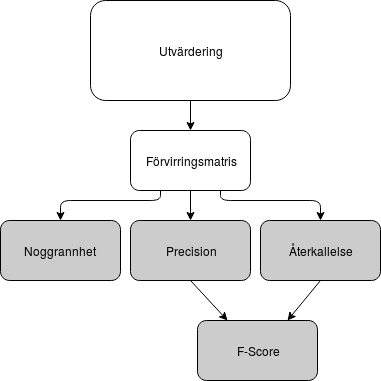
\includegraphics[width=10cm]{utvardering}
\centering
\caption{Utvärderingsmetoder för TSA.}
\label{fig:utv}
\end{figure}


\section{Sammanfattning} \label{BACKsum}
I detta kapitel har bakgrunden till projektet diskuterats där nyttan av SA och TSA har tagits upp. Intressant för uppdragsgivaren är hur de kan integrera SA och TSA i sina produkter t.ex. chatbotar och trendanalys. 

Detta kapitel ger även en överblick vad maskininlärning är och hur maskininlärnings viktigaste komponenterna hänger ihop samt hur maskininlärning kan appliceras på SA och TSA. Dessutom beskrivs de problem och utmaningar som existerar inom TSA. 

\chapter{Experiment}
\section{Intro}
\section{Bearbetning av datamängd} \label{exp:pre}
\section{Särdragsurval} \label{exp:feat}
\section{Algoritmer}
\subsection{Naive Bayes}
\subsection{Support Vector Machine}
\newpage
\section{Implementation}
\subsection{Naive Bayes}
\subsection{Support Vector Machine}
\subsection{Prediction program.}
\subsection{* ev GUI implementation om tid finns *}
\section{Sammanfattning}

\chapter{Resultat}
\section{Intro}
\section{Resultatet mellan modellerna}
\subsection{Dataset 1 -> jämför resultat mellan modellerna}
\subsection{Dataset 2 -> jämför resultat mellan modellerna}
\subsection{Dataset 3 -> jämför resultat mellan modellerna}
\newpage
\section{Implementations mässigt vilken modell är lättast?}
\section{implementations jämförelse (resultat VS förväntat)}
\section{Summering}

\chapter{Slutsats}
\section{Sammanfattning}
\section{Problem}
\section{Begränsningar}
\newpage
\section{Vidare utveckling}
\section{Slutord}



\bibliographystyle{unsrtnat} 
\bibliography{../refs/thesisref}


\restoregeometry%

\end{document}
\endinput
%%
%% End of file `kaumasterstemplate.tex'.
